\documentclass[prodmode]{acmsmall-ec14}

% Package to generate and customize Algorithm as per ACM style
\usepackage[ruled]{algorithm2e}
\renewcommand{\algorithmcfname}{ALGORITHM}
\SetAlFnt{\small}
\SetAlCapFnt{\small}
\SetAlCapNameFnt{\small}
\SetAlCapHSkip{0pt}
\IncMargin{-\parindent}

%\conferenceinfo{EC'14,}{June 8--12, 2014, Stanford, CA, USA.}
%\CopyrightYear{2014}
%\crdata{978-1-4503-2565-3/12/06}
%\copyrighttext{Copyright is held by the owner/author(s). Publication rights licensed to ACM.}

\doi{2600057.2602898}% TeXSupport
\clubpenalty=10000
\widowpenalty = 10000

%% Metadata Information
%\acmVolume{X}
%\acmNumber{X}
%\acmArticle{X}
%\acmYear{2014}
%\acmMonth{2}
%\usepackage[numbers]{natbib}

\usepackage{environ}
\usepackage{color}
\usepackage{amsmath,amsfonts,amssymb}
\usepackage{verbatim}
\usepackage{graphicx}
\usepackage{subfigure}
\usepackage{multirow}
%\usepackage[capitalise]{cleveref}
%\usepackage{tikz}
\usepackage{caption}
%%%%%%%%%%%%%%%%%%%%%%%%%%%%%%%%%%%%%%%%%%%%%
%%%%%%%%%%%%%%%%%%%%%%%%%%%%%%%%%%%%%%%%%%%%%
%%%%%%%%%%%%%%%%%%%%%%%%%%%%%%%%%%%%%%%%%%%%%

\newcommand{\X}{\ensuremath{\mathcal{X}}}
\newcommand{\R}{\ensuremath{\mathcal{R}}}
\newcommand{\mP}{\ensuremath{\mathcal{P}}}
\newcommand{\mM}{\ensuremath{\mathcal{M}}}
\newcommand{\ip}[2]{\ensuremath{\langle #1, #2 \rangle}}
\newcommand{\grad}{\nabla}
\newcommand{\one}{\ensuremath{\mathbf{1}}}
\newcommand{\co}{\mbox{co}}

\newcommand{\calL}{{\mathcal{L}}}
\newcommand{\rank}{{\calL(A)}}
\newcommand{\calO}{{\mathcal{O}}}
\newcommand{\calP}{{\mathcal{P}}}

\newcommand{\uni}{{\rank^n}}

\DeclareMathOperator*{\argmax}{arg\,max}
\DeclareMathOperator*{\argmin}{arg\,min}
\newcommand{\eps}{\epsilon}
\newcommand{\ones}{\mathbf{1}}

\newtheorem{claim}[theorem]{Claim}
\newtheorem{observation}[theorem]{Observation}
%\newtheorem{theorem}{Theorem}
%\newtheorem{lemma}{Lemma}
%\newtheorem{conjecture}{Conjecture}
%\newtheorem{proposition}{Proposition}
%\newtheorem{corollary}{Corollary}
%
%\newenvironment{definition}[1][Definition]{\begin{trivlist}
%\item[\hskip \labelsep {\bfseries #1}]}{\end{trivlist}}
%\newenvironment{example}[1][Example]{\begin{trivlist}
%\item[\hskip \labelsep {\bfseries #1}]}{\end{trivlist}}
%\newenvironment{remark}[1][Remark]{\begin{trivlist}
%\item[\hskip \labelsep {\bfseries #1}]}{\end{trivlist}}


\newcount\Comments
\Comments=1
\newcommand{\kibitz}[2]{\ifnum\Comments=1\textcolor{#1}{#2}\fi}
\renewcommand{\sl}[1]{\kibitz{blue} {[SL: #1]}}
\newcommand{\ns}[1]{\kibitz{red} {[NS: #1]}}

\newcommand{\nt}{NT}

% Document starts
\begin{document}

% Page heads
%\markboth{Lahaie and Shah}{Neutrality and Geometry of Mean Voting}

% Title portion
\title{Neutrality and Geometry of Mean Voting}
\author{
S\'{e}bastien Lahaie
\affil{Microsoft Research, New York City, United States.}
Nisarg Shah
\affil{Carnegie Mellon University, Pittsburgh, United States.}
}

\begin{abstract}
Mean proximity rules provide a simple geometric framework to achieve consensus among a collection of rankings (votes) over a set of alternatives. They embed all rankings into a Euclidean space, take the mean of the embeddings of the input votes, and return the ranking whose embedding is closest to the mean. Previous work on mean proximity rules has not integrated an important axiom---neutrality---into the framework. By drawing on ideas from the representation theory of finite groups, we show that integrating neutrality actually helps achieve a succint representation for \emph{every} mean proximity rule. Various connections are drawn between mean proximity rules and other prominent approaches to social choice.
\end{abstract}

\category{I.2.6}{Computing Methodologies}{Artificial Intelligence}
\category{J.4}{Computer Applications}{Social and Behavioral Sciences}[Economics]

%\terms{Algorithms, Economics}

\keywords{Social choice, Mean proximity rules, Euclidean space, Neutrality}

%\acmformat{S\'{e}bastien Lahaie and Nisarg Shah, 2014. Neutrality and Geometry of Mean Voting.}

\begin{bottomstuff}
Shah was visiting and partially supported by Microsoft Research New York City during the course of this work.

Author's addresses:  S. Lahaie, Microsoft Research New York City, \url{slahaie@microsoft.com}; N. Shah, Computer Science Department, Carnegie Mellon, \url{nkshah@cs.cmu.edu}.
\end{bottomstuff}

\maketitle
\section{Introduction}
\label{sec:intro}

Modern social choice literature has seen rising interest in studying families of voting rules for aspects like manipulability~\cite{Gib73,Sat75,Xia13} and learnability~\cite{PZR08,PZPR09}. Particularly, the framework of \emph{generalized scoring rules} (GSRs)~\cite{XC08} has been a great success in this direction. Two other well-studied approaches---\emph{distance rationalizability}~\cite{MN08,EFS09,elkind2010good} and \emph{maximum likelihood estimation} (MLE)~\cite{Con85,Young88,CS05b}---have given rise to many families of voting rules as well. More recently, Caragiannis et al.~\shortcite{CPS13} introduced the families of PM-c and PD-c rules as generalizations of Condorcet consistent rules and positional scoring rules, respectively. Their goal was to design rules that perform well in predicting an underlying ground truth from noisy data. 

These families of voting rules are extremely general in that generalized scoring rules, distance rationalizable rules, MLE rules, as well as the union of PM-c and PD-c rules contain \emph{almost all} voting rules. Consequently, interesting restrictions of such families have been studied in the literature~\cite{CPS14,EFS09,elkind2010good,CS05b}. 

%\ns{However, these approaches have been rather unfruitful because the definition of these families depend on the choices of a distance metric over permutations and a noise model for generating noisy estimates of a ground truth, respectively; these choices can be extremely general, thus both families end up suffering from the aforementioned problem of containing \emph{almost all} voting rules.}

The family of \emph{mean proximity rules} introduced by Zwicker~\shortcite{Zwicker08a} is one such restriction; it is a proper subset of each of generalized scoring rules, distance rationalizable rules, and maximum likelihood estimators (see Section~\ref{sec:connection}). Additionally, each rule in the family does what a voting rule should intuitively do: aggregate the input votes into a mean consensus. A plethora of voting rules have emerged due to the fact that there is no natural notion of \emph{mean} of a set of rankings. Mean proximity rules embed rankings into a Euclidean space, and use the natural mean (in the Euclidean space) of the embeddings of the input votes to guide the consensus. When this mean does not represent embedding of any ranking, the ranking whose embedding is closest to the mean is chosen as the consensus. Different ways to embed the rankings into the Euclidean space give rise to different mean proximity rules. In this sense, mean proximity rules use Euclidean spaces to achieve the mean representative of the input votes. Examples of mean proximity rules include the Kemeny rule and all positional scoring rules. 

{\footnotesize
\begin{figure}
\centering
\subfigure[The Borda count for $3$ alternatives]{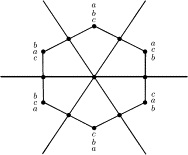
\includegraphics[width=0.25\textwidth]{images/borda.jpg}\label{fig:borda}}\qquad
\subfigure[The Kemeny rule for $3$ alternatives]{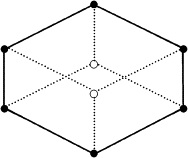
\includegraphics[width=0.25\textwidth]{images/kemeny.jpg}\label{fig:kemeny}}
\caption{Geometric visualizations of mean proximity rules}
\label{fig:geometric}
\end{figure}
}

Consider the embedding given in Figure~\ref{fig:borda}\footnote{Credit:~\cite{ovchinnikov2005hyperplane}} that generates the Borda count for $3$ alternatives. The $6$ rankings are embedded into the vertices of a regular hexagon. Each voter adds a unit weight to the vertex corresponding to his vote, and the ranking whose region contains the mean (the center of gravity) of all the votes is chosen as the output. For a simulation of this process using rubber bands, see \url{http://omega.math.union.edu/research/2010-05-voting/}. Similarly, Figure~\ref{fig:kemeny} shows the embedding generating the Kemeny rule for $3$ alternatives. Mean proximity rules provide an easy understanding and in some cases simple visualizations of voting rules (even of the Kemeny rule that is usually considered a black-box algebraic problem). Saari~\shortcite{saari1995basic} argues that such a clear understanding is crucial for a voting rule to be accepted in the real-world, even more so for positional rules\footnote{By positional rules, we mean rules that pay attention to alternatives in all positions of the input votes.} that are arguably more complex than simple rules such as plurality or $k$-approval. He then makes a compelling case of using geometry in order to clarify and visualize voting rules. However, the geometric intuitions behind mean proximity rules are fundamentally different from those in Saari's work. 

Despite the attractive outlook, mean proximity rules have received less attention in the literature. We tap the potential and uncover significant structures in mean proximity rules. When introducing mean proximity rules, Zwicker~\shortcite{Zwicker08a} was motivated to remove neutrality primarily due to the characterization by Myerson~\shortcite{Myerson95} that all social choice functions (voting rules that output a single winning alternative) satisfying neutrality, consistency, and another mild axiom are scoring rules. However, we study mean proximity rules in the context of social welfare functions, for which consistency is significantly weaker. Hence, neutrality can be integrated without much loss; e.g., the Kemeny rule is retained along with positional scoring rules. On the other hand, we show that integrating neutrality has several benefits.

\noindent \textbf{Our contributions.} Mean proximity rules have two alternative representations, one geometric and one algebraic. We study mean proximity rules in a slightly limited context of social welfare functions, and characterize the constraints the limited context imposes on both representations (Theorem~\ref{thm:symm}). Next, we study the important axiom of neutrality in the framework of mean proximity rules. 

We give a characterization of the constraints imposed by neutrality on both representations of mean proximity rules (Theorem~\ref{thm:neutral-smpr}). In this context, we introduce \emph{neutral embeddings}, and show that every neutral mean proximity rule admits a neutral embedding. By drawing ideas from the representation theory of finite groups, we further introduce \emph{linear embeddings}, and show that every neutral mean proximity rule also admits a linear embedding. Linear embeddings are more constructive in nature, and thus have additional benefits over neutral embeddings. While storing a $k$-dimensional embedding for each of $m!$ rankings typically takes $O(k \cdot m!)$ space, linear embeddings leverage group theoretic structure to reduce the space requirement to $O(k^2)$. This provides a succint representation for every neutral mean proximity rule, which distinguishes the family of low-dimensional neutral mean proximity rules from the other families of voting rules mentioned in the introduction where storing a rule requires exponential space in the worst case. 

Using a fairly technical but constructive proof, in Theorem~\ref{thm:neutral-linear} we establish that (almost) every neutral embedding is also a linear embedding, and its succinct representation can also be computed. This leads to a new characterization of neutral mean proximity rules that yields further side results such as a characterization of mean proximity rules that admit low-dimensional embeddings. We conclude by drawing connections between mean proximity rules and various lines of research in social choice literature, showing that mean proximity rules connect well with each line of research. 

\section{Related Work}
\label{sec:related}

We build upon the work of Zwicker~\shortcite{Zwicker08a,Zwicker08b} who introduced and studied mean proximity rules and their generalization called mean neat rules, and gave an axiomatic characterization of (rational) mean neat voting rules. The work of Cervone et al.~\shortcite{CDGL+12} builds upon mean proximity rules and utilizes another notion of geometric consensus known as mediancenter or the Fermat-Weber point. They use the intuition of a rubber band and each voter exerting force to bring the consensus close to himself which is similar to the intuition behind mean proximity rules. 

The work of Saari~\shortcite{saari1995basic} uses a different geometric visualization where a profile is viewed in the space of $m!$ dimensions, each dimension encoding the number of times a particular ranking appears in a given profile. Daugherty et al.~\shortcite{daugherty2009voting} extend his work by using intricate results from group representation theory. Related lines of research also include the work of Brams and Fishburn~\shortcite{brams2007approval} that argue in favor of approval voting for its simplicity and clarity, and the work of Crisman~\shortcite{permuta} that connects the Borda count and the Kemeny rule using the geometry of permutahedron --- the mean proximity embedding of the Borda count that is similar to Figure~\ref{fig:borda} but for $4$ alternatives. Note that in these lines of research (as well as in this paper), the Euclidean space is merely used as a tool to understand voting rules, and does not bear any intrinsic meaning.

%These lines of research must be separated from the models~\cite{} where the alternatives are embedded into a Euclidean space, and voters preferences are expressed as points in the same Euclidean space; the Euclidean space used in these models and the embeddings of the alternatives have specific meaning whereas the former lines of research use the Euclidean space merely as a tool to understand the voting rules.

\section{Preliminaries}
\label{sec:prelim}
Let $A$ be the set of alternatives, with cardinality $|A| = m$. Let $\rank$ denote the set of rankings over the alternatives in $A$. A profile $\pi \in \rank^n$ is a collection of votes (rankings). A \emph{voting rule}, or more technically a \emph{social welfare function} (SWF), is a function that maps every profile to a ranking or set of tied rankings.\footnote{Another common definition of a voting rule is a \emph{social choice function} (SCF), which maps every profile to a winning alternative or set of tied alternatives.} Formally, we denote a voting rule by $r : \rank^n \rightarrow \calP(\rank)\setminus\{\emptyset\}$, where $\calP(\cdot)$ denotes the power set. Note that a voting rule must output at least one ranking so $\emptyset$ is disallowed. 

%For any profile $\pi$, let $n(\pi,\sigma)$ denote the number of times $\sigma$ appears in $\pi$. Let $\sigma_1,\ldots,\sigma_{m!}$ denote a fixed reference order of the rankings in $\rank$. For any two profiles $\pi_1$ and $\pi_2$, let $\pi_1+\pi_2$ be the union profile such that $n(\pi_1+\pi_2,\sigma) = n(\pi_1,\sigma)+n(\pi_2,\sigma)$ for every $\sigma \in \rank$. Similarly, for any profile $\pi$, let $c \pi$ be the profile such that $n(c \pi,\sigma) = c \cdot n(\pi,\sigma)$ for every $\sigma \in \rank$. 

\subsection*{Axiomatic Properties} Voting rules are often studied (and sometimes designed) from the viewpoint of axiomatic properties. Such properties prescribe the behavior of a voting rule in certain special cases. Some widely studied properties of relevance to our work are defined below. 

\begin{description}
\item[Anonymity] A voting rule $r$ is called \emph{anonymous} if its output only depends on the collection of rankings in the profile (equivalently, the number of times each ranking appears), and not on the identities of the voters providing the different rankings. \\ %For every profiles $\pi_1$ and $\pi_2$ such that $n(\pi_1,\sigma) = n(\pi_2,\sigma)$ for every $\sigma \in \rank$, $r(\pi_1) = r(\pi_2)$.

\item[Consistency] A voting rule $r$ is called \emph{consistent} if for profiles $\pi_1$ and $\pi_2$ such that $r(\pi_1) \cap r(\pi_2) \neq \emptyset$, we have $r(\pi_1+\pi_2) = r(\pi_1) \cap r(\pi_2)$.\footnote{Consistency for social welfare functions that output a set of tied rankings is more general than consistency for social welfare functions that output a single ranking (i.e., a singleton set). It is also significantly different from consistency of the winning alternative for social choice functions.} Here, profile $\pi_1+\pi_2$ denotes the union of the profiles $\pi_1$ and $\pi_2$. \\ %A social welfare function $r$ is called weakly consistent (for rankings) if for every profiles $\pi_1$ and $\pi_2$ such that $r(\pi_1) = r(\pi_2)$, we have $r(\pi_1+\pi_2) = r(\pi_1) = r(\pi_2)$. 

\item[Unanimity] A voting rule $r$ is said to satisfy \emph{unanimity} if on every profile $\pi$ that consists of copies of a single ranking $\sigma$, the rule uniquely outputs that ranking, so that $r(\pi) = \{\sigma\}$.\\ %the singleton set uniquely outputs that ranking: for every profile $\pi$ such that $n(\pi,\sigma) > 0$ for some $\sigma \in \rank$ and $n(\pi,\sigma') = 0$ for all $\sigma' \neq \sigma$, $r(\pi) = \{\sigma\}$. 

\item[Rank-distinguishability] A voting rule $r$ satisfies rank-distinguishability if for every two distinct rankings $\sigma, \sigma' \in \rank$, there must exist a profile $\pi$ such that exactly one of $\sigma$ and $\sigma'$ belongs to $r(\pi)$. 
\end{description}

\noindent
In the classical definition of social welfare functions that output a single ranking, non-imposition (also known as citizen sovereignty) of a voting rule dictates that every ranking of the alternatives should be achievable as the output of the voting rule on some profile. The rank-distinguishability axiom is a mild generalization of non-imposition to social welfare functions that output a set of rankings. It follows from unanimity which is itself considered unrestrictive and almost always desirable.

The next axiom will be central to our study. Let us choose the labels of the alternatives to be $1,2,\ldots,m$. A relabeling of the alternatives is equivalent to a permutation of $[m]$, namely an element of the symmetric group $S_m$. For a permutation $\tau \in S_m$ and a ranking $\sigma \in \rank$, the ranking $\tau\sigma$ is obtained by relabeling the alternatives according to $\tau$ in $\sigma$. Given a profile $\pi = (\sigma_1,\ldots,\sigma_n)$ and a permutation $\tau$ of the alternatives, let $\tau \pi = (\tau \sigma_1,\ldots,\tau \sigma_n)$ be the profile where each vote is permuted according to $\tau$. Similarly, given any set of rankings $S$, let $\tau S = \{\tau \sigma : \sigma \in S\}$.
%
\begin{description}
\item[Neutrality] A voting rule $r$ is \emph{neutral} if for every profile $\pi$ and permutation $\tau$ of the alternatives, we have $r(\tau \pi) = \tau r(\pi)$.
\end{description}
%
In words, a voting rule is called neutral if the labels of the alternatives do not matter, i.e., relabeling the alternatives would relabel the output of the rule (each ranking in the set returned) accordingly.  

\subsection*{Voting Rules} Next, we define two prominent voting rules that play a key role in this paper.

\begin{description}
\item[Kemeny rule] Given a profile $\pi$, define the weighted pairwise majority (PM) graph of $\pi$ as the graph where the alternatives are the vertices and, for every pair of alternatives $a$ and $b$, there is a directed edge from $a$ to $b$ with weight equal to the number of voters that prefer $a$ to $b$. The Kemeny score of a ranking $\sigma$ is the total weight of the edges in the PM graph of $\pi$ whose direction agrees with $\sigma$. The Kemeny rule selects the ranking or set of tied rankings with the highest Kemeny score.\\

\item[Positional scoring rules] A positional scoring rule is given by a scoring vector $\alpha = (\alpha_1,\ldots,\alpha_m) \in \mathbb{R}^m$ where $\alpha_i \ge \alpha_{i+1}$ for all $i \in [m]$ and $\alpha_1 > \alpha_m$. Under this rule, for each vote $\sigma$ in $\pi$ and $i \in [m]$, $\alpha_i$ points are awarded to the $i${th} most preferred alternative in $\sigma$. The rule returns set of all rankings where the alternatives are sorted in descending order of total points. Some examples of positional scoring rules include plurality, Borda count, veto, and $k$-approval.
\end{description}

%ns - Connectedness is not used much. No need to define here. 
%\begin{definition}[Connectedness]
%A voting rule $r$ is called \emph{connected} if for any two profiles $\pi_1$ and $\pi_2$ with $r(\pi_1) \cap r(\pi_2) \neq \emptyset$, there exist non-negative integers $c$ and $d$ such that $r(\pi_1) \cap r(c \pi_1 + d \pi_2) \neq \emptyset$ and $r(\pi_1) \neq r(c \pi_1 + d \pi_2)$. 
%\end{definition}

%%%%%%%%%%%%%%%%%%%%%%%%%%%%%%%%%%%%%%%%%%%%%

%\ns{Check if this is equivalent/related to continuity defined by Conitzer et al.~\cite{CRX09}. Then we can add that to Proposition~\ref{prop:properties}.}
%\begin{definition}[Continuity]
%Two profiles $\pi_1$ and $\pi_2$ satisfy $\pi_1 \approx \pi_2$ if they differ by one vote: for some $\sigma$ and $\sigma'$, $n(\pi_1,\sigma) = n(\pi_2,\sigma)-1$, $n(\pi_1,\sigma') = n(\pi_2,\sigma')+1$, and for every $\sigma \in \rank\setminus\{\sigma,\sigma'\}$, $n(\pi_1,\sigma) = n(\pi_2,\sigma)$. A voting rule $r$ is called \emph{continuous} if for every profile $\pi$ and ranking $\sigma$, $\sigma \notin r(\pi)$ implies that there exists integer $k$ such that for every profile $\pi' \approx k \pi$, $\sigma \notin r(\pi')$. 
%\end{definition}

\section{Mean Proximity Rules}
\label{sec:mpr}

We begin by  presenting important background on mean proximity rules that will be relevant for the rest of the paper. Mean proximity rules were originally defined in a scope greater than that of the voting rules considered in this paper: While voting rules map every profile to a set of tied rankings, mean proximity rules in general map every profile to a set of tied outcomes, where the outcomes are chosen from a generic outcome space $\calO$. In Section~\ref{sec:symm}, we will fix $\calO = \rank$ to analyze mean proximity rules in the context of voting rules. Here and throughout, $\|\cdot\| $ refers to the Euclidean norm.

\begin{definition}[Mean Proximity Rules~\cite{Zwicker08a}]
A \emph{mean proximity rule} is given by an input embedding $\phi: \rank \rightarrow \mathbb{R}^k$ mapping input rankings to $k$-dimensional Euclidean space and an output embedding $\psi: \calO \rightarrow \mathbb{R}^k$ mapping possible outcomes to the same Euclidean space. The outcome of the rule on a profile $\pi$ is given by the set $\argmin_{o \in \calO} \|\psi(o) - \mu(\pi) \|$, where $\mu(\pi) = (1/n) \cdot \sum_{\sigma \in \pi} \phi(\sigma)$ is the mean of input embeddings of the votes in $\pi$, and $\|\cdot\|$ is the Euclidean norm.\footnote{In this paper, every summation of the form $\sum_{\sigma \in \pi}$  iterates over rankings in profile $\pi$; in particular, if a ranking appears multiple times in $\pi$, the summation contains one term for each appearance.}
\end{definition}

\noindent
Zwicker~\shortcite{Zwicker08a} also defined another family of rules, which he referred to as \emph{generalized scoring rules}. However, this name has since been used primarily to represent a different family of voting rules that was introduced by Xia and Conitzer~\shortcite{XC08}. We therefore refer to the family of Zwicker~\shortcite{Zwicker08a} as \emph{matrix scoring rules}. In Section~\ref{sec:connection}, we observe that the family of matrix scoring rules introduced by Zwicker~\shortcite{Zwicker08a} is a subset of the family of generalized scoring rules introduced by Xia and Conitzer~\shortcite{XC08}. 

\begin{definition}[Matrix Scoring Rules~\cite{Zwicker08a}]
A voting rule is called a \emph{matrix scoring rule} if there exists a scoring function $s : \rank \times \calO \rightarrow \mathbb{R}$ such that for any profile $\pi$, we have $r(\pi) = \argmax_{o \in \calO} \sum_{\sigma \in \pi} s(\sigma,o)$. 
\end{definition}

%%%%%%%%%%%%%%%%%%%%%%%%%%%%%%%%%%%%%%%%%%%%%

%\begin{proposition}[Corollary~4.2.3, Zwicker~\cite{Zwicker08a}]
%Let $A = \{u_1,\ldots,u_l\}$ be a set of $l$ vectors in $\mathbb{R}^k$. Let $B = \{v_1,\ldots,v_p\}$ be a set of $p$ vectors in $\mathbb{R}^k$. Then, the discrete mean in $A$ of vectors in $B$ is the vector in $A$ that is closest to the Euclidean mean of vectors in $B$. That is,
%$$
%\argmin_{u_i \in A} \sum_{v_j \in B} \|u_i - v_j\|^2 = \argmin_{u_i \in A} \|u_i - (1/p) \cdot \sum_{v_j \in B} v_j\|.
%$$
%\label{prop:discrete-mean}
%\end{proposition}

\noindent
In words, the matrix scoring rule assigns a score to each outcome for each input vote, and the outcome or outcomes with the highest aggregate score are chosen. Our choice of terminology stems from the fact that the scoring function can be represented as a $|\calL| \times |\calO|$ matrix with real entries. Zwicker~\shortcite{Zwicker08a} also showed equivalence between mean proximity rules and matrix scoring rules using the following technical result. %We reconstruct his proof because it is crucial to several proofs in this paper. 

\begin{proposition}[\cite{Zwicker08a}]
For embeddings $\phi : \rank \rightarrow \mathbb{R}^k$ and $\psi: \calO \to \mathbb{R}^k$, and profile $\pi$, we have
\begin{equation}
\argmin_{o \in \calO} \|\psi(o)-\mu(\pi)\| = \argmin_{o \in \calO} \sum_{\sigma \in \pi} \|\psi(o)-\phi(\sigma)\|^2.
\label{eqn:discrete-mean}
\end{equation}
\label{prop:MPR-GSR-conversion}
\end{proposition}
%\begin{comment}
%\begin{proof}[Proof (reconstructed)]
%\begin{align*}
%&\argmin_{o \in \calO} \|\psi(o)-\mu(\pi)\| \\
%&\quad= \argmin_{o \in \calO} \|\psi(o)-\mu(\pi)\|^2 \\
%&\quad= \argmin_{o \in \calO} \|\psi(o)\|^2 + \|\mu(\pi)\|^2 - 2 \cdot \langle \psi(o), (1/n) \sum_{\sigma \in \rank} n(\pi,\sigma) \phi(\sigma) \rangle\\
%&\quad= \argmin_{o \in \calO} n \cdot \|\psi(o)\|^2 - 2 \sum_{\sigma \in \rank} n(\pi,\sigma) \cdot \langle \psi(o), \phi(\sigma) \rangle\\
%&\quad= \argmin_{o \in \calO} \sum_{\sigma \in \rank} n(\pi,\sigma) \cdot (\|\psi(o)\|^2 - 2 \cdot \langle \psi(o), \phi(\sigma) \rangle )\\
%&\quad= \argmin_{o \in \calO} \sum_{\sigma \in \rank} n(\pi,\sigma) \cdot (\|\psi(o)\|^2 - 2 \cdot \langle \psi(o), \phi(\sigma) \rangle + \|\phi(\sigma)\|^2)\\
%&\quad= \argmin_{o \in \calO} \sum_{\sigma \in \rank} n(\pi,\sigma) \cdot \|\psi(o)-\phi(\sigma)\|^2.
%\end{align*}
%\end{proof}
%\end{comment}
%
From the definition of matrix scoring rules and Proposition~\ref{prop:MPR-GSR-conversion}, it is clear that the scoring function $s(\sigma,o) = -\|\psi(o)-\phi(\sigma)\|^2$ represents the same mean proximity rule that has the embeddings $(\psi,\phi)$. Extending this to a two-way correspondence, Zwicker~\shortcite{Zwicker08a} showed the following. 
\begin{proposition}[{\cite[Theorem 4.2.1]{Zwicker08a}}]
The families of mean proximity rules and matrix scoring rules coincide. 
\label{prop:equiv}
\end{proposition}
%\begin{comment}
%\begin{proof}[Proof (reconstructed)]
%Take any mean proximity rule $r$. Let $\phi$ and $\psi$ be any input and output embeddings that generate $r$. Using Proposition~\ref{prop:MPR-GSR-conversion}, we can see that $r$ is a matrix scoring rule with the score function $s(\sigma,o) = -\|\psi(o)-\phi(\sigma)\|^2$. 
%
%For the other direction, take any matrix scoring rule $r$ and let $s$ be any score function that generates $r$. Then, let $\phi(\sigma) = (s(\sigma,o_1),\ldots,s(\sigma,o_k))$ where $\{o_1,\ldots,o_k\}$ is some fixed enumeration of $\calO$. Further, let $\psi(o_i) = e_i \in \mathbb{R}^k$ where the $i^{th}$ coordinate is $1$ and the rest are $0$. Then, for any profile $\pi$, we have
%\begin{align*}
%o_i \in r(\pi) &\Leftrightarrow \sum_{\sigma \in \rank} n(\pi,\sigma) \cdot s(\sigma,o_i) \ge \sum_{\sigma \in \rank} n(\pi,\sigma) \cdot s(\sigma,o), \forall o \in \calO\\
%&\Leftrightarrow \langle \mu(\pi), e_i \rangle \ge \langle \mu(\pi), e_j \rangle, \forall 1 \le j \le k \\
%&\Leftrightarrow \|\mu(\pi) - e_i\| \ge \|\mu(\pi) - e_j\|, \forall 1 \le j \le k\\
%&\Leftrightarrow \|\mu(\pi) - \psi(o_i)\|^2 \ge \|\mu(\pi) - \psi(o_j)\|^2, \forall 1 \le j \le k,\\
%&\Leftrightarrow \|\mu(\pi) - \psi(o_i)\| \ge \|\mu(\pi) - \psi(o_j)\|, \forall 1 \le j \le k,
%\end{align*}
%where the third transition follows since $\|e_j\| = 1$ for all $j$ (and thus, $\|\mu(\pi) - \psi(o_j)\|^2 - \langle \mu(\pi), e_j \rangle$ is constant for all $j$). Thus, $r$ is a mean proximity rule.
%\end{proof}
%\end{comment}

%%%%%%%%%%%%%%%%%%%%%%%%%%%%%%%%%%%%%%%%%%%%%
\noindent
According to this result, a mean proximity rule has two equivalent representations: a pair of embeddings $(\psi,\phi)$, and a scoring function $s$; it may be the case that neither of the two is unique. We conclude the background on mean proximity rules by mentioning a result of Zwicker~\shortcite{Zwicker08b} that further motivates the study of mean proximity rules.

%\ns{What about the characterization given in the related paper?}
\begin{proposition}[\cite{Zwicker08b}]
All positional scoring rules and the Kemeny rule are mean proximity rules, with the outcome space being the set of rankings over the alternatives. A mean proximity rule is consistent, connected, continuous, and anonymous.
\label{prop:properties}
\end{proposition}
%
Consistency of mean proximity rules is evident from Equation~\eqref{eqn:discrete-mean} because if two profiles lead to overlapping outputs according to the rule, then this overlap minimizes the sum on the right-hand side of Equation~\eqref{eqn:discrete-mean} for each profile, and therefore for their union. Connectedness and continuity are two natural properties of voting rules defined in~\cite{Zwicker08a}. For an alternative, but related, definition of continuity, the reader may refer to~\cite{CRX09}. Conitzer and Sandholm~\shortcite{CS05b} showed that other rules such as Bucklin's rule, Copeland's method, the maximin rule, and the ranked pairs method are not consistent as social welfare functions. Hence, these rules are not mean proximity rules. 

%%%%%%%%%%%%%%%%%%%%%%%%%%%%%%%%%%%%%%%%%%%%%
%%%%%%%%%%%%%%%%%%%%%%%%%%%%%%%%%%%%%%%%%%%%%
%%%%%%%%%%%%%%%%%%%%%%%%%%%%%%%%%%%%%%%%%%%%%

\subsection{Symmetric Mean Proximity Rules}
\label{sec:symm}

We now begin our investigation of mean proximity rules in the context of social welfare functions that output rankings over alternatives. Thus, from here onwards, we fix $\calO = \rank$. This has the following effect on the various equivalent representations of mean proximity rules.
\begin{enumerate}
\item The embeddings $\phi,\psi : \rank \to \mathbb{R}^k$ both map rankings to a Euclidean space. 
\item The scoring function $s : \rank \times \rank \rightarrow \mathbb{R}$ describes \emph{similarity} between two rankings. This special case was also defined and studied independently by Conitzer et al.~\shortcite{CRX09}, who referred to such rules as \emph{simple ranking scoring functions} (SRSFs). 
\item Under a fixed enumeration $\sigma_1,\ldots,\sigma_{m!}$ of $\rank$, we can represent a scoring function by an $m! \times m!$ \emph{score matrix} $S$ such that $S_{ij} = s(\sigma_i,\sigma_j)$ for $i,j \in [m!]$.
\end{enumerate}
%
Mean proximity rules constitute a broad family of voting rules, some of which violate natural desiderata. For example, a mean proximity rule given by a scoring function $s$ that satisfies $s(\sigma,\sigma') > s(\sigma,\sigma)$ for distinct $\sigma,\sigma' \in \rank$ would not output $\sigma$ even on the profile where all the votes are $\sigma$, violating unanimity. To solve this problem, we propose a simple adjustment. 

\begin{definition}[Symmetric Mean Proximity Rule]
We say that a voting rule is a \emph{symmetric mean proximity rule} (SMPR) if there exists a mean proximity representation of the rule with identical input and output embeddings: $\psi = \phi$. 
\end{definition} 
%
Since the outcome space for SWFs is identical to the space of input votes (the set of rankings over the alternatives), $\psi = \phi$ is a natural restriction. Note that not all embeddings representing an SMPR satisfy $\psi = \phi$. We call the embeddings that satisfy this restriction \emph{symmetric embeddings}. From here onwards, we always represent an SMPR using a symmetric embedding $(\phi$, $\phi)$, written simply $\phi$.

In what follows, we assume that the SMPRs additionally satisfy rank-distinguishability. For SMPRs, rank-distinguishability is equivalent to the intuitive restriction that $\phi$ must map all rankings to different points of the Euclidean space. To see this, note that if $\phi$ mapped all rankings to distinct points, then the rule would output $\{\sigma\}$ on a profile with a single vote $\sigma$. Thus, such a rule would achieve rank-distinguishability. Conversely, if $\phi$ mapped two distinct rankings $\sigma$ and $\sigma'$ to the same point in the Euclidean space, then it is easy to see that on every profile either both rankings would belong to the output of the rule or neither. 

%\footnote{We slightly abuse the notation by referring to $\phi(\sigma)$ as the embedding of $\sigma$ under $\phi$.} 

\begin{observation}
An SMPR satisfies rank-distinguishability if and only if every symmetric embedding $\phi$ representing the rule maps all rankings to distinct points of the Euclidean space.
\end{observation}
%
Under this assumption, it is easy to check that in a profile $\pi$ where all the votes are $\sigma$, we have $\mu(\pi) = \phi(\sigma)$. As a result, the output of every symmetric mean proximity rule on $\pi$ would be the singleton set $\{\sigma\}$. Therefore, not only does symmetry impose intuitive structure on mean proximity rules, it also helps achieve natural desiderata such as unanimity. Furthermore, the embeddings constructed in~\cite{Zwicker08a} for positional scoring rules and the Kemeny rule in fact satisfy the restriction $\psi = \phi$, showing that these canonical mean proximity rules are symmetric. 

%\begin{lemma}
%While there exist mean proximity rules violating unanimity, all symmetric mean proximity rules satisfy unanimity.
%\end{lemma}
%

%\begin{lemma}
%All positional scoring rules and the Kemeny rule are symmetric mean proximity rules.
%\label{lem:symmetric-captures}
%\end{lemma}


%%%%%%%%%%%%%%%%%%%%%%%%%%%%%%%%%%%%%%%%%%%%%

\subsection{Algebraic Characterization of Symmetry}
\label{sec:smpr-char}

Recall that mean proximity rules are equivalent to matrix scoring rules (Proposition~\ref{prop:equiv}). In the previous section we imposed symmetry on the embeddings of the mean proximity rules. It is therefore natural to ask: \emph{What restriction does symmetry place on other equivalent representations of mean proximity rules}? For an embedding $\phi$, define the scoring function $s_{\phi}$ such that $s_{\phi}(\sigma,\sigma') = -\|\phi(\sigma)-\phi(\sigma')\|^2$ for all $\sigma,\sigma' \in \rank$. Then Equation~\eqref{eqn:discrete-mean} implies that $s_{\phi}$ and $\phi$ are equivalent, meaning they both represent the same SMPR. Further, the score matrix generated by $s_{\phi}$ has a well-known structure.

%%%%%%%%%%%%%%%%%%%%%%%%%%%%%%%%%%%%%%%%%%%%%

\begin{definition}[Euclidean Distance Matrix]
A $q \times q$ matrix $A = (a_{ij})$ is called a \emph{Euclidean distance matrix (EDM)} if there exist $v_1,\ldots,v_q \in \mathbb{R}^p$ $(p \leq q)$ such that $a_{ij} = \|v_i-v_j\|^2$ for all $i,j \in [q]$. 
\end{definition}
%
A matrix $A$ is \emph{conditionally positive semidefinite} if $x^T A x \geq 0$ for all vectors $x$ such that $\ones^T x = 0$, where $\ones = (1,1,\ldots,1)$. It is known that a non-negative matrix with zero diagonal entries is a negated EDM if and only if it is conditionally positive definite; see~\cite[Thm 3.10]{ikramov2000conditionally} and~\cite{schoenberg1938metric}.

By construction, the score matrix of $s_{\phi}$ is a negated EDM and represents the given SMPR.  Conversely, given any score matrix that is a negated EDM, by definition we can find a symmetric embedding $\phi$ such that the score matrix is generated by the scoring function $s_{\phi}$. Hence, the rule represented by the score matrix must be an SMPR. This yields the following characterization. 
%
\begin{theorem}
A voting rule is a symmetric mean proximity rule if and only if it is a matrix scoring rule whose score matrix is a negated Euclidean Distance Matrix, or equivalently, a non-negative, conditionally positive semidefinite matrix with zero diagonal entries.
\label{thm:symm}
\end{theorem}
%\begin{proof}
%Take any symmetric mean proximity rule $r$. Let $\phi$ be arbitrary embedding of $r$, and let $s_{\phi}$ be its equivalent scoring function. Then it is easy to observe that the score matrix of $s_{\phi}$ is, by definition, negation of an EDM. Alternatively, given any score matrix that is negation of an EDM, by definition we can find an embedding $\phi$ such that the score matrix is generated by the scoring function $s_{\phi}$. Hence, the rule is a symmetric mean proximity rule.
%\begin{comment} % Full Proof
%For the ``if'' direction, given any matrix scoring rule $r$ with score matrix $S$ such that $-S$ is an EDM, we can find $v_1,\ldots,v_{m!} \in \mathbb{R}^k$ such that $S_{ij} = -\|v_i-v_j\|^2$. Take $\phi(\sigma_i) = v_i$ for all $i$. By Proposition~\ref{prop:MPR-GSR-conversion}, 
%$$
%\argmax_{\sigma \in \rank} \sum_{\sigma' \in \rank} n(\pi,\sigma') \cdot s(\sigma,\sigma') = \argmin_{\sigma \in \rank} \|\phi(\sigma)-\mu(\pi)\|.
%$$
%That is, the rule is a symmetric mean proximity rule. For the ``only if'' direction, given any symmetric mean proximity rule, note that the score matrix created in the proof of Proposition~\ref{prop:equiv} is negation of a Euclidean distance matrix.
%\end{comment}
%\end{proof}
%
Note that while mean proximity SWFs coincide with the family of matrix scoring rules (i.e. simple ranking scoring functions) due to Conitzer et al.~\shortcite{CRX09}, our focus on \emph{symmetric} mean proximity rules gives a fairly non-trivial algebraic condition on the score matrix that translates to a rather intuitive geometric condition in the alternative mean proximity representation. 

To summarize, we provided two motivations for adding symmetry to mean proximity rules: (1) taking identical input and output embeddings reflects the fact that the outcome space coincides with the space of input votes in the case of voting rules, and (2) symmetric mean proximity rules achieve the additional requirement of unanimity while still capturing all well-known mean proximity rules. We then characterized symmetric mean proximity rules in three equivalent representations: embeddings in Euclidean space, scoring functions, and score matrices. In the next section, we provide characterizations under the addition of another desirable property, \emph{neutrality}. While neutrality is also a mild requirement (all voting rules of interest are neutral), we show that it adds significant structure to mean proximity rules. 

%%%%%%%%%%%%%%%%%%%%%%%%%%%%%%%%%%%%%%%%%%%%%
%%%%%%%%%%%%%%%%%%%%%%%%%%%%%%%%%%%%%%%%%%%%%
%%%%%%%%%%%%%%%%%%%%%%%%%%%%%%%%%%%%%%%%%%%%%

\section{Neutrality and Symmetric Mean Proximity Rules}
\label{sec:neutrality}
Recall that neutrality of a voting rule states that the labels of the alternatives do not matter: relabeling alternatives relabels the output in the same fashion. We remark that our analysis of mean proximity rules focuses on understanding the way voting rules work \emph{before} they break ties. Therefore, mean proximity rules output a set of tied results (in our case, rankings over the alternatives), and do not explicitly break ties. Note that most rules do not remain neutral after lexicographic tie-breaking is imposed, but are neutral (as per the definition in this paper) before ties are broken. Further, uniformly random tie-breaking (where each tied result is returned with equal probability) can always be used to retain neutrality even after tie-breaking. 

In Section~\ref{sec:charact}, we study the restrictions imposed by neutrality on the various equivalent representations of \emph{symmetric} mean proximity rules. We connect neutrality of SMPRs with a notion of neutrality in the embedding, a similar notion of neutrality in the scoring function~\cite{CRX09}, and positive semidefiniteness of the score matrix. In Section~\ref{sec:linear}, we give a constructive characterization by drawing ideas from group representation theory. 

\subsection{Characterizations of Neutrality}
\label{sec:charact}

We begin by defining neutrality of scoring functions as in~\cite{CRX09}. 

\begin{definition}[Neutral Scoring Function]
A scoring function $s: \rank \times \rank \rightarrow \mathbb{R}$ is called \emph{neutral} if $s(\tau \sigma, \tau \sigma') = s(\sigma,\sigma')$ for all rankings $\sigma,\sigma' \in \rank$ and permutations $\tau \in S_m$. We say that a score matrix is neutral if its underlying scoring function is neutral. 
\end{definition}
In words, a scoring function is neutral if the similarity between two rankings given by the function does not change when both rankings are permuted in the same way. Conitzer et al.~\shortcite{CRX09} showed that any scoring function $s$ of a neutral mean proximity rule $r$ can be converted to an equivalent neutral scoring function.

\begin{proposition}[\cite{CRX09}] Let $s$ be a scoring function representing a mean proximity rule $r$ that is neutral. Then, an equivalent neutral scoring function $s^{\nt}$ representing the same rule $r$ can be defined as follows. For all rankings $\sigma,\sigma' \in \rank$ and permutations $\tau \in S_m$, let
\begin{equation}
s^{\nt}(\sigma,\sigma') = \sum_{\tau \in S_m} s(\tau \sigma, \tau \sigma').
\label{eqn:s-nt}
\end{equation}
\label{prop:neutral-scoring}
\end{proposition}
%
Additionally, it is easy to check that by definition every neutral scoring function represents a neutral mean proximity rule. We immediately obtain the following.
 
\begin{proposition}[{\cite[Lemma~2]{CRX09}}]
A mean proximity rule is neutral if and only if it is represented by a neutral scoring function.
\label{prop:gsr-neutral}
\end{proposition}
%
%\noindent \textbf{What does this mean for us?}
This proposition characterizes the conditions on the scoring function (and thus on the score matrix) that neutrality imposes on mean proximity rules. However, we are interested in the addition of neutrality to \emph{symmetric} mean proximity rules. Together with Theorem~\ref{thm:symm}, Proposition~\ref{prop:gsr-neutral} implies that a voting rule is a symmetric mean proximity rules if and only if it has a neutral score matrix and a score matrix that is negation of an EDM. \emph{Is there a score matrix satisfying both conditions?} \emph{What conditions does neutrality impose on the embedding of an SMPR?} To answer these questions, we first introduce a notion of neutrality for an embedding.



\begin{definition}[Neutral Embedding]
We say that an embedding $\phi:\rank \rightarrow \mathbb{R}^k$ is \emph{neutral} if for all rankings $\sigma,\sigma' \in \rank$ and permutations $\tau \in S_m$, we have $\|\phi(\sigma)-\phi(\sigma')\| = \|\phi(\tau \sigma)-\phi(\tau\sigma')\|$.
\end{definition}
%
It can be checked that if the embedding $\phi$ is neutral, then its corresponding score function $s_{\phi}$ is also neutral. Further, similarly to scoring functions, an embedding can also be neutralized. 

\begin{lemma}
Let $\phi: \rank \to \mathbb{R}^k$ be an embedding of an SMPR $r$. Then, $\phi^{\nt}$ defined as follows is an equivalent neutral embedding of the same SMPR $r$: 
\begin{equation}
\phi^{\nt}(\sigma) = [\phi(\tau_1 \sigma)^T \phi(\tau_2 \sigma)^T \ldots \phi(\tau_{m!} \sigma)^T]^T,
\label{eqn:phi-nt}
\end{equation}
where $\tau_1,\ldots,\tau_{m!}$ is a fixed enumeration of the permutations in $S_m$. Further, the neutralization of $\phi$ and the neutralization of its scoring function $s_{\phi}$ are connected via $s_{\phi^{\nt}} = s ^{\nt}_{\phi}$, where the neutral scoring function $s ^{\nt}_{\phi}$ defined in~\eqref{eqn:s-nt} represents $r$. 
\label{lem:neutral-embedding}
\end{lemma}
\begin{proof}
First, we show that $\phi^{\nt}$ is neutral. For all rankings $\sigma,\sigma' \in \rank$ and permutations $\tau \in S_m$, 
\begin{align*}
\|\phi^{\nt}(\tau \sigma)-\phi^{\nt}(\tau \sigma')\|^2 &= \sum_{\tau' \in S_m} \|\phi(\tau' \tau \sigma)-\phi(\tau' \tau \sigma)\|^2 \\
&= \sum_{\tau' \in S_m} \|\phi(\tau' \sigma)-\phi(\tau' \sigma)\|^2 = \|\phi^{\nt}(\sigma)-\phi^{\nt}(\sigma)\|^2,
\end{align*}
where the second equality holds because for $\tau \in S_m$, we have $\{\tau' \tau : \tau' \in S_m\} = S_m$, which is a property of any group. Hence, $\phi^{\nt}$ is neutral. Next, for all rankings $\sigma,\sigma' \in \rank$, 
\begin{align*}
s_{\phi^{\nt}}(\sigma,\sigma') = -\|\phi^{\nt}(\sigma)-\phi^{\nt}(\sigma')\|^2 &= - \sum_{\tau \in S_m} \|\phi(\tau \sigma)-\phi(\tau \sigma')\|^2  \\
&= \sum_{\tau \in S_m} s_{\phi}(\tau \sigma,\tau \sigma') = s_{\phi}^{\nt}(\sigma,\sigma').
\end{align*}
Thus, we have $s_{\phi^{\nt}} = s_{\phi}^{\nt}$. The scoring function $s_{\phi}$ is equivalent to the embedding $\phi$, and thus also represents the rule $r$. From Proposition~\ref{prop:neutral-scoring}, the scoring function $s_{\phi}^{\nt} = s_{\phi^{\nt}}$ also represents $r$. Hence, the embedding $\phi^{\nt}$ also represents $r$. 
\end{proof}
%
We remark that the neutralized embedding $\phi^{\nt}$ is not very satisfactory because it maps rankings to a Euclidean space with dimension $m!$ times the dimension used by $\phi$. (Of course, as there are only $m!$ rankings, the embeddings lie on a subspace of dimension at most $m!$)
However, it has significant structure. For example, in addition to neutrality we also have $\|\phi^{\nt}(\sigma)\|^2 = \sum_{\tau \in S_m} \|\phi(\tau \sigma)\|^2 = \sum_{\sigma' \in \rank} \|\phi(\sigma')\|^2$. 
Hence, $\|\phi^{\nt}(\sigma)\|$ is independent of $\sigma$. That is, $\phi^{\nt}$ is an \emph{equal norm embedding}.
%
\begin{definition}[Equal Norm Embedding]
We say that an embedding $\phi : \rank \rightarrow \mathbb{R}^k$ has \emph{equal norm} if $\|\phi(\sigma)\| = \|\phi(\sigma')\|$ for all rankings $\sigma,\sigma' \in \rank$.
\end{definition}
%
For equal norm embeddings, squares of Euclidean distances in Proposition~\ref{prop:MPR-GSR-conversion} can be replaced by inner products as follows.
\begin{lemma}
For an equal norm embedding $\phi$ of an SMPR $r$, the scoring function $s$ given by $s(\sigma,\sigma') = \langle \phi(\sigma),\phi(\sigma') \rangle$ for all rankings $\sigma,\sigma' \in \rank$ represents $r$. 
\label{lem:inner-product}
\end{lemma}
\begin{proof}
Let the equal norm embedding $\phi$ have $\|\phi(\sigma)\| = c$ for all $\sigma \in \rank$. From Proposition~\ref{prop:MPR-GSR-conversion}, we know that on a profile $\pi$, 
\begin{align*}
r(\pi) &= \argmin_{\sigma \in \rank} \sum_{\sigma' \in \pi} \|\phi(\sigma)-\phi(\sigma')\|^2 \\
&= \argmin_{\sigma \in \rank} \sum_{\sigma' \in \pi} \left( c^2 + c^2 - 2 \langle \phi(\sigma), \phi(\sigma')\rangle\right) \\
&= \argmin_{\sigma \in \rank}\: 2 c^2\cdot m! - 2 \sum_{\sigma' \in \pi} \langle \phi(\sigma), \phi(\sigma')\rangle = \argmax_{\sigma \in \rank} \sum_{\sigma' \in \pi} \langle \phi(\sigma), \phi(\sigma')\rangle.
\end{align*}
Hence, by definition $s$ is a scoring function representing $r$. 
\end{proof}
%
The score matrix generated by the inner product scoring function of Lemma~\ref{lem:inner-product} has a well-known structure. 
\begin{definition}[Gram Matrix]
A $q \times q$ matrix $A = (a_{ij})$ is called a \emph{Gram matrix} if there exist vectors $v_1,\ldots,v_q \in \mathbb{R}^p$ $(p \leq q)$ such that $a_{ij} = \langle v_i,v_j \rangle$ for all $i,j \in [q]$. It is well-known that a matrix is Gramian if and only if it is positive semidefinite. 
\end{definition}
%
Recall that a matrix $A$ is \emph{positive semidefinite} if $x^T A x \geq 0$ for all vectors $x$. It is a standard fact that a matrix is a Gram matrix if and only if it is positive definite. 
With this machinery at hand, we are ready to answer the questions we posed regarding conditions on various representations of an SMPR imposed by neutrality. 
%We present the answer in the form of the following characterization.
%\begin{theorem}
%A voting rule is a neutral symmetric mean proximity rule if and only if it is a matrix scoring rule that has a score matrix which is neutral, positive semidefinite, and has equal diagonal entries. 
%\label{thm:neutral-psd}
%\end{theorem}
%\begin{proof}
%Take any neutral symmetric mean proximity rule $r$. By Theorem~\ref{thm:linear-char}, it has a linear embedding $\phi$. Consider its normalization $\hat{\phi}$, which is also linear by Lemma~\ref{lem:preservation}. Next, consider the Gramian matrix (and hence positive semidefinite) $S$ of $\hat{\phi}$, which is a score matrix of $r$ due to Lemma~\ref{lem:inner-product}.  Using the fact that linear embeddings are equal norm neutral embeddings (Lemma~\ref{lem:linear-neutral}) and Lemma~\ref{lem:inner-products-preserve}, we can see that $\langle \hat{\phi}(\tau \sigma), \hat{\phi}(\tau \sigma') \rangle = \langle \hat{\phi}(\sigma), \hat{\phi}(\sigma') \rangle$ for all $\tau,\sigma,\sigma' \in \rank$. Hence, $S$ is also neutral. Further, equal norm property of $\hat{\phi}$ implies that $S$ has equal diagonal entries. 
%
%Conversely, take any matrix scoring rule $r$ with a score matrix $S$ that is neutral, positive semidefinite, and has equal diagonal entries. Since $S$ is positive semidefinite, it is also Gramian. Then, we can find vectors $v_1,\ldots,v_{m!}$ such that $S_{ij} = \langle v_i,v_j \rangle$. Take $\phi(\sigma_i) = v_i$. Equal diagonal entries of $S$ imply that $\phi$ has equal norm. Hence, $\phi$ is an equal norm embedding whose Gramian matrix is a score matrix of $r$. Hence, $r$ is a symmetric mean proximity rule with embedding $\phi$. Further, it is easy to see that neutrality of $S$ and equal norm property of $\phi$ imply neutrality of $\phi$, which in turn implies neutrality of $r$. 
%\end{proof}

%%%%%%%%%%%%%%%%%%%%%%%%%%%%%%%%%%%%%%%%%%%%%

\begin{theorem}
For a mean proximity rule $r$, the following are equivalent. 
\begin{enumerate}
\item $r$ is neutral and symmetric.
\item There exists a neutral symmetric embedding representing $r$.
\item There exists a non-negative score matrix representing $r$ which is neutral, conditionally positive semidefinite, and has zero diagonal entries. 
\item There exists a score matrix representing $r$ which is neutral, positive semidefinite, and has equal diagonal entries.
\end{enumerate}
\label{thm:neutral-smpr}
\end{theorem}
\begin{proof}
It is easy to show that the second and the third conditions imply the first condition. If $r$ has a score matrix satisfying the third conditions, namely it is a negated EDM, then by Proposition~\ref{prop:gsr-neutral} and Theorem~\ref{thm:symm}, $r$ is a neutral SMPR. Similarly, if $r$ is a symmetric mean proximity rule with a neutral embedding $\phi$, then for a profile $\pi$, we have 
\begin{align*}
r(\tau \pi) &= \argmin_{\sigma \in \rank} \sum_{\sigma' \in \pi} \|\phi(\sigma)-\phi(\tau \sigma')\|^2 \\
&= \tau \; \argmin_{\sigma \in \rank} \sum_{\sigma' \in \pi} \|\phi(\tau \sigma)-\phi(\tau \sigma')\|^2 \\
&= \tau \; \argmin_{\sigma \in \rank} \sum_{\sigma' \in \pi} \|\phi(\sigma)-\phi(\sigma')\|^2 = \tau r(\pi),
\end{align*}
where the first transition follows from Proposition~\ref{prop:MPR-GSR-conversion}, and the third transition follows from neutrality of $\phi$. Thus, $r$ is a neutral SMPR. 

Conversely, let $r$ be a neutral SMPR and $\phi$ be its embedding. We proved in Lemma~\ref{lem:neutral-embedding} that $s_{\phi}^{\nt} = s_{\phi^{\nt}} = s$ (say). Then, $s = s_{\phi}^{\nt}$ implies that the score matrix corresponding to the scoring function $s$ is neutral. Further, $s = s_{\phi^{\nt}}$ implies that the score matrix is also a negated EDM. Hence, the score matrix corresponding to the scoring function $s$ is both neutral and a negated EDM, implying the third condition. Further, the equivalent embedding $\phi^{\nt}$ is neutral and represents $r$, implying the second condition. Thus, we have shown that the first three conditions are equivalent. 

For equivalence with the fourth condition, take a neutral SMPR $r$ and its embedding $\phi$. We saw that the embedding $\phi^{\nt}$ has equal norm, and hence the score matrix $S$ corresponding to its scoring function $s$ given by $s(\sigma,\sigma') = \langle \phi^{\nt}(\sigma),\phi^{\nt}(\sigma')\rangle$ is a Gram score matrix representing $r$ (Lemma~\ref{lem:inner-product}). Since $S$ is a Gram matrix, it is also positive semidefinite. The equal norm property of $\phi^{\nt}$ implies that $S$ has equal diagonal entries. Finally, neutrality of $\phi^{\nt}$ implies neutrality of $S$. Hence, $S$ satisfies the requirements of the fourth condition. 

Conversely, take a mean proximity rule $r$ with a score matrix $S$ that is neutral, positive semidefinite, and has equal diagonal entries. Then, we can find an embedding $\phi$ such that $S$ is its Gram matrix. Neutrality and equal diagonal entries of $S$ imply neutrality and the equal norm property of $\phi$. The latter implies that $\phi$ also represents $r$ (Lemma~\ref{lem:inner-product}). Hence, $r$ must be a neutral SMPR. 
\end{proof}

%TOADD: We point out that more properties could be proven for the score matrix $S$ constructed in the proof of Theorem~\ref{thm:neutral-smpr} for any given neutral symmetric mean proximity rule (which is the Gramian of a normalized linear embedding $\hat{\phi}$). In addition to being neutral and positive semidefinite, and having equal diagonal entries, the sum of entries along each row and column of $S$ is also zero. To see this, note that $\hat{\phi}_{avg} = 0$. Hence, the sum of entries of $S$ across row $i$ or column $i$ is $m! \cdot \langle \hat{\phi}(\sigma_i), \hat{\phi}_{avg} \rangle = 0$. Another interesting factoid is that existence of a score matrix that is both neutral and positive semidefinite with equal diagonal entries can be established alternatively by taking any score matrix that is positive semidefinite and has equal diagonal entries (Gramian of any normalized embedding), and then neutralizing it by the construction of Conitzer et al.~\cite{CRX09} given in Equation~\eqref{eqn:s-nt}.

%It is worthwhile pointint out that following steps very similar to those in the proof of Theorem~\ref{thm:neutral-smpr}, one can also show that a mean proximity rule (not necessarily symmetric) is neutral if and only if it has a representation in which both input and output embeddings are neutral. 
\noindent
Theorem~\ref{thm:neutral-smpr} translates neutrality of an SMPR to neutrality of its embedding. While it is straightforward to check whether a given embedding is neutral, generating neutral embeddings is a non-trivial task. This limits the constructiveness of the characterization. Next, we improve the characterization by showing that neutrality of an embedding is equivalent to a structure that provides a way to generate neutral embeddings. 
%%%%%%%%%%%%%%%%%%%%%%%%%%%%%%%%%%%%%%%%%%%%%
%%%%%%%%%%%%%%%%%%%%%%%%%%%%%%%%%%%%%%%%%%%%%
%%%%%%%%%%%%%%%%%%%%%%%%%%%%%%%%%%%%%%%%%%%%%

\subsection{Linear Embeddings}
\label{sec:linear}

Group representation theory has played a important role in a diverse set of fields including %\footnote{See \url{http://wdjoyner.com/repn_thry_appl.html} for a wider range of applications.} 
coding theory, quantum mechanics, and crystallography (in chemistry)~\cite{BR86,KHS93,MS77}. A linear representation of a group essentially maps every group element to a linear transformation of a vector space, i.e., to an element of the general linear group on the vector space. When a basis is chosen for the vector space, the linear transformation can be represented via a matrix. This is known as matrix representation of a group. 

In our case, we draw on the representation theory of the symmetric group, which has gained much attention and for which many interesting structures have been discovered leveraging the extreme symmetry of the group~\cite{JKCR84}. We fix the standard Euclidean basis for simplicity. We now introduce \emph{linear embeddings} using ideas from linear representations of the symmetric group. 

%%%%%%%%%%%%%%%%%%%%%%%%%%%%%%%%%%%%%%%%%%%%%

\begin{definition}[Linear Embeddings]
We say that an embedding $\phi:\rank \rightarrow \mathbb{R}^k$ is \emph{linear} if there exists a representation function $R : S_m \rightarrow \mathbb{R}^{k \times k}$, called the representation of $\phi$, mapping each permutation to a $k \times k$ real matrix such that 
\begin{enumerate}
\item the identity permutation $\tau_e$ is mapped to the identity matrix: $R(\tau_e) = I_k$,
\item $R$ respects the multiplication operator of the symmetric group: $R(\tau_1 \tau_2) = R(\tau_1) R(\tau_2)$ for all permutations $\tau_1,\tau_2 \in S_m$ (where $\tau_1 \tau_2$ represents the multiplication of $\tau_1$ and $\tau_2$ within $S_m$), 
\item $R$ maps permutations to orthogonal matrices: $R(\tau)^T = R(\tau)^{-1}$ for all permutations $\tau \in S_m$, and
\item permuting a ranking is equivalent to rotating---because $R$ uses orthogonal matrices---its embedding appropriately: $\phi(\tau \sigma) = R(\tau) \phi(\sigma)$ for all rankings $\sigma \in \rank$ and permutations $\tau \in S_m$.
\end{enumerate}
\end{definition}

\noindent
It can be easily seen that the first and the second conditions together imply that $R(\tau^{-1}) = R(\tau)^{-1}$ for all permutations $\tau \in S_m$, where $\tau^{-1}$ is the inverse of $\tau$ in $S_m$. Further, the third condition is completely unrestrictive: A striking result from group representation theory states that for a representation $R$ of any finite group (not just the symmetric group), there exists a matrix $P$ such that the equivalent representation $R'$ defined by $R'(g) = P R(g) P^{-1}$ for each group element $g$ uses orthogonal matrices; see, e.g.,~\cite[Thm~6.3]{BMWM63}. That is, any representation can be converted to a representation that uses orthogonal matrices. In what follows, we use $R_{\tau}$ instead of $R(\tau)$ for notational convenience. 

Before we dive into the equivalence between neutrality and linearity, we build its pillars by presenting a few results about linear embeddings. 
\begin{lemma}
For a linear embedding $\phi$, rankings $\sigma,\sigma' \in \rank$, and permutation $\tau \in S_m$, we have
$$
\langle \phi(\tau \sigma), \phi(\tau \sigma') \rangle = \langle \phi(\sigma), \phi(\sigma') \rangle.
$$
\label{lem:inner-product-preserve}
\end{lemma}
\begin{proof}
Let $R$ be the representation of $\phi$. Then, we have 
\begin{equation}
\langle \phi(\tau \sigma), \phi(\tau \sigma') \rangle = \langle R_{\tau}\phi(\sigma), R_{\tau}\phi(\sigma') \rangle = \langle \phi(\sigma), R_{\tau}^T R_{\tau}\phi(\sigma') \rangle = \langle \phi(\sigma), \phi(\sigma') \rangle,
\label{eqn:linear-inner-product}
\end{equation}
where, the last transition holds because $R_{\tau}$ is an orthogonal matrix by definition. 
\end{proof}
%
Taking $\sigma = \sigma'$ in Lemma~\ref{lem:inner-product-preserve}, we get the following corollary.
%
\begin{corollary}
Every linear embedding has equal norm.
\label{cor:linear-equal-norm}
\end{corollary}
%
While every linear embedding has equal norm, not every neutral embedding has equal norm. However, the next result shows that every neutral embedding has a similar equal distance property. The proof considers a profile where each ranking appears exactly once; a detailed proof is given in the full version of the paper.\footnote{Full version of the paper is available at \url{http://www.cs.cmu.edu/~nkshah/euclidean_voting.full.pdf}}

\begin{lemma}
Let $\phi$ be a neutral embedding, and $\phi_{avg} = (1/m!) \cdot \sum_{\sigma \in \rank} \phi(\sigma)$ denote the mean embedding of all rankings under $\phi$. Then, $\|\phi(\sigma)-\phi_{avg}\|$ is a constant independent of the ranking $\sigma$.
\label{lem:average-all}
\end{lemma}
%
Given Lemma~\ref{lem:average-all}, we can easily derive an equal norm embedding given a neutral embedding: Given a neutral embedding $\phi$, we say that the embedding $\hat{\phi}$ defined by $\hat{\phi}(\sigma) = \phi(\sigma) - \phi_{avg}$ for all $\sigma \in \rank$ is the \emph{normalization} of $\phi$. Note that $\hat{\phi}$ is simply a translation applied to $\phi$, which is distance-preserving. Hence, $\hat{\phi}$ represents the same neutral SMPR as $\phi$ does. This normalization achieves the equal norm property (Lemma~\ref{lem:average-all}), and also preserves neutrality and linearity of the original embedding. The proof is straightforward and given in the full version of the paper. %appendix.

%%%%%%%%%%%%%%%%%%%%%%%%%%%%%%%%%%%%%%%%%%%%%

\begin{lemma}
An embedding is neutral (resp.\ linear) if and only if its normalization is neutral (resp.\ linear). 
\label{lem:preservation}
\end{lemma}
%
Lemma~\ref{lem:preservation} shows that the normalization of a neutral embedding is also neutral, in addition to having the equal norm property. We now show that this normalization is in fact linear---this requires a much deeper proof. 

\begin{theorem}
An embedding is neutral if and only if its normalization is linear. 
\label{thm:neutral-linear}
\end{theorem}
\begin{proof}
We first show that a linear embedding is also a neutral embedding. Let $\phi$ be a linear embedding. Then for all $\sigma,\sigma' \in \rank$ and $\tau \in S_m$, we have
\begin{align*}
\|\phi(\tau \sigma)-\phi(\tau \sigma')\|^2 &= \|\phi(\tau \sigma)\|^2 + \|\phi(\tau \sigma')\|^2 - 2\cdot \langle \phi(\tau \sigma), \phi(\tau \sigma') \rangle \\
&= \|\phi(\sigma)\|^2 + \|\phi(\sigma')\|^2 - 2\cdot \langle \phi(\sigma), \phi(\sigma') \rangle = \|\phi(\sigma)-\phi(\sigma')\|^2,
\end{align*}
where the second transition holds due to Lemma~\ref{lem:inner-product-preserve} and its Corollary~\ref{cor:linear-equal-norm}. Thus, $\phi$ is also neutral. 

Now, for our main result, let $\phi$ be an embedding whose normalization $\hat{\phi}$ is linear. Then, $\hat{\phi}$ is also neutral as shown above. Due to Lemma~\ref{lem:preservation}, this implies that $\phi$ is also neutral.

The converse is much trickier, therefore we provide the high-level overview of the proof. Take a neutral embedding $\phi : \rank \rightarrow \mathbb{R}^k$, and let $r$ be the rule it represents. We want to show that $\hat{\phi}$ is linear. By Corollary~\ref{cor:linear-equal-norm} and Lemma~\ref{lem:preservation}, we know that $\hat{\phi}$ is a ($k$-dimensional) equal norm neutral embedding. We first construct an equivalent embedding $\phi^f$ as follows. Let $k' \le k$ be the dimension of the affine subspace of $\mathbb{R}^k$ spanned by the points $\{\hat{\phi}(\sigma)\}_{\sigma \in \rank}$. Then, we obtain $\phi^f$ by taking a distance-preserving mapping to $\mathbb{R}^{k'}$. Next, we show that $\phi^f$ is linear by explicitly constructing its representation using Moore-Penrose pseudoinverses. Finally, we use this to construct an explicit representation for $\hat{\phi}$ itself. 

Now we provide the formal proof. First, it is easy to check that $\hat{\phi}_{avg} = 0$. Hence, the affine space spanned by the embeddings under $\hat{\phi}$ form a linear subspace of $\mathbb{R}^k$ of dimension $k'$. Take an orthonormal basis $v_1,\ldots,v_{k'}$ of this linear subspace, write $\hat{\phi}(\sigma)$ as a linear combination of the $k'$ basis vectors, and let $\phi^f(\sigma)$ encode the coefficients of the linear combination. Equivalently, if $P$ is the $k' \times k$ matrix with $v_1,\ldots,v_{k'}$ as its rows, then $\phi^f(\sigma) = P \phi(\sigma)$ for all $\sigma \in \rank$. It is now standard to show that the transformation $P$ preserves all distances. This has two implications: First, $\phi^f$ represents the same neutral SMPR $r$ as $\hat{\phi}$ and $\phi$ do. Second, $\phi^f$ is also an equal norm neutral embedding like $\hat{\phi}$. These hold because the definitions of mean proximity rules, equal norm property, and neutrality of embeddings only use distances between pairs of embeddings. 

By construction, $\phi^f$ is of \emph{full dimension}, i.e., the points where the rankings are mapped span the whole of $\mathbb{R}^{k'}$.\footnote{While it is not relevant for the proof, we remark that the fact that the $m!$ points span $\mathbb{R}^{k'}$ implies $k' \le m!$.} Next, consider the matrix $A = [\phi^f(\sigma_1), \ldots, \phi^f(\sigma_{m!})]$, the $k' \times m!$ matrix whose columns are the embeddings under $\phi^f$. Here, $\sigma_1,\ldots,\sigma_{m!}$ is an enumeration of $\rank$. This implies that $A$ must have full row rank $k'$. Fix a permutation $\tau \in S_m$, and consider $B = [\phi^f(\tau \sigma_1), \ldots, \phi^f(\tau \sigma_{m!})]$. Then for all $i,j \in [m!]$, 
$$
(B^T B)_{ij} = \langle \phi^f(\tau \sigma_i), \phi^f(\tau \sigma_j) \rangle = \langle \phi^f(\sigma_i), \phi^f(\sigma_j) \rangle = (A^T A)_{ij}
$$
where the second transition follows because $\phi^f$ is neutral. Thus, $A^T A = B^T B$.

We now show that there exists a matrix $R_{\tau}$ such that $\phi^f(\tau \sigma) = R_{\tau} \phi^f(\sigma)$ for all $\sigma \in \rank$. Combining the equations for all $\sigma \in \rank$, it is equivalent to show the existence of an $R_{\tau}$ such that $R_{\tau} A = B$, i.e., existence of a solution $X$ of the linear system $A^T X = B^T$. It is well-known that the system of equations $Ax=b$ has a solution if and only if $AA^{+}b = b$, where $A^{+}$ is the Moore-Penrose pseudoinverse of $A$ (see, e.g.,~\cite{BH12}). Trivially extending this to multiple systems of linear equations, we can see that the necessary and sufficient condition for existence of the required $R_{\tau}$ is $A^T (A^T)^{+} B^T = B^T$, or equivalently, $B A^{+} A = B$. The last derivation uses the fact that $(A^T)^{+} = (A^{+})^T$. Now, 
\begin{align*}
B &= B B^{+} B = B \left( (B^T B)^{+} B^T \right) B = B (B^T B)^{+} \left( B^T B \right) \\
&= B (A^T A)^{+} \left( A^T A \right) = B \left( (A^T A)^{+} A^T \right) A = B A^{+} A.
\end{align*}
Refer~\cite{BH12} for the identities $X = X X^{+} X$ (used in the first transition) and $X^{+} = (X^T X)^{+} X^T$ (used in the second and the fifth transitions) regarding Moore-Penrose pseudoinverses. The fourth transition holds because $A^T A = B^T B$. Hence, we have shown that for every permutation $\tau \in S_m$, there exists a matrix $R_{\tau}$ such that $\phi^f(\tau \sigma) = R_{\tau} \phi^f(\sigma)$ for all $\sigma \in \rank$. Further, one solution of $Ax=b$ is $x = A^{+}b$. Extending this, we can see that one solution of $A^T X = B^T$ is $X = (A^T)^{+} B^T$. Hence, $R_{\tau} = X^T = BA^{+}$. We choose this particular solution for every $\tau \in S_m$ and show that it satisfies the conditions of linearity. 

Recall that the rank of the product of two matrices is at most the minimum of the rank of the two matrices, and $R_{\tau} A = B$. Also, both $A$ and $B$ are rank $k'$ matrices. Hence, $rank(R_{\tau}) \ge k'$. However, $R_{\tau}$ is a $k' \times k'$ matrix. Hence, we conclude that $R_{\tau}$ is invertible for every $\tau \in S_m$. We now show that $R_{\tau_1 \tau_2} = R_{\tau_1} R_{\tau_2}$ for all $\tau_1,\tau_2 \in S_m$. 

Fix $\tau_1,\tau_2 \in S_m$. For every $\sigma \in \rank$, we have $\phi^f(\tau_1 \tau_2 \sigma) = R_{\tau_1 \tau_2} \phi^f(\sigma)$. Also, $\phi^f(\tau_1 \tau_2 \sigma) = R_{\tau_1} \phi^f(\tau_2 \sigma) = R_{\tau_1}R_{\tau_2} \phi^f(\sigma)$. Thus, we have that $R_{\tau_1 \tau_2} \phi^f(\sigma) = R_{\tau_1} R_{\tau_2} \phi^f(\sigma)$ for all $\sigma \in \rank$. It is easy to show that this implies $R_{\tau_1 \tau_2} = R_{\tau_1} R_{\tau_2}$. To see this, consider the submatrix of $A$---let us call it $A_p$---by taking $k'$ linearly independent columns of $A$. Then, $A_p$ is an invertible square matrix. Also, $R_{\tau_1 \tau_2} A_p = R_{\tau_1} R_{\tau_2} A_p$. Multiplying by $A_p^{-1}$ on both sides, we get the desired result. To complete the proof, we need to show that $R_{\tau}$ is an orthogonal matrix for all $\tau \in S_m$, i.e., $R_{\tau}^{-1} = R_{\tau}^T$. Note that 
$$
R_{\tau}^T B = (A^{+})^T B^T B = (A^{+})^T A^T A = (A A^{+})^T A = I A = A,
$$
where the second transition holds because $B^T B = A^T A$, and the fourth transition holds because $A A^{+} = I$ for any full row-rank matrix $A$ (see, e.g.,~\cite{BH12}). Thus, we have that $R_{\tau}^T B = A$. Applying $R_{\tau}$ on both sides, we get $R_{\tau} R_{\tau}^T B = R_{\tau} A = B$. Similarly to $A_p$, we can construct an invertible submatrix $B_p$ of $B$, and get $R_{\tau} R_{\tau}^T B_p = B_p$, which, upon right-multiplication by $B_p^{-1}$, yields the required equation $R_{\tau}^{-1} = R_{\tau}^T$. Thus, $\phi^f$ is a linear embedding. We now show that $\hat{\phi}$ is also linear. 

Consider the orthonormal basis $v_1,\ldots,v_{k'}$ that was used for constructing $\phi^f$ from $\hat{\phi}$, and the corresponding matrix $P$ with $v_i$'s as its rows. Complete this to a basis $v_1,\ldots,v_k$ of $\mathbb{R}^k$, and consider the matrix $Q$ that has all the $v_i$'s as its rows. Then, $Q \hat{\phi}(\sigma) = [\phi^f(\sigma)^T, 0, \ldots, 0]^T$, where the number of zeros is $k-k'$. For a permutation $\tau \in S_m$, construct the $k \times k$ matrix 
$$
R'_{\tau} = Q^T \left[ \begin{smallmatrix} R_{\tau} & 0 \\ 0 & I \end{smallmatrix} \right] Q. 
$$
Here, $R_{\tau}$ is a $k' \times k'$ matrix and $I$ is the $(k-k') \times (k-k')$ identity matrix. Note that 
$$
R'_{\tau} \hat{\phi}(\sigma) = Q^T \left[ \begin{smallmatrix} R_{\tau} & 0 \\ 0 & I \end{smallmatrix} \right] Q \hat{\phi}(\sigma) = Q^T \left[ \begin{smallmatrix} R_{\tau} & 0 \\ 0 & I \end{smallmatrix} \right] [\phi^f(\sigma) 0 \ldots 0]^T = Q^T [\phi^f(\tau \sigma)^T, 0, \ldots, 0]^T = \hat{\phi}(\tau \sigma).
$$
Thus, $R'_{\tau} \hat{\phi}(\sigma) = \hat{\phi}(\tau \sigma)$ for all $\tau \in S_m$ and $\sigma \in \rank$. Further, 
\begin{align*}
R'_{\tau_1} R'_{\tau_2} &= Q^T \left[ \begin{smallmatrix} R_{\tau_1} & 0 \\ 0 & I \end{smallmatrix} \right] Q Q^T \left[ \begin{smallmatrix} R_{\tau_2} & 0 \\ 0 & I \end{smallmatrix} \right] Q = Q^T \left[ \begin{smallmatrix} R_{\tau_1} & 0 \\ 0 & I \end{smallmatrix} \right] \left[ \begin{smallmatrix} R_{\tau_2} & 0 \\ 0 & I \end{smallmatrix} \right] Q \\
&= Q^T \left[ \begin{smallmatrix} R_{\tau_1} R_{\tau_2} & 0 \\ 0 & I \end{smallmatrix} \right] Q = Q^T \left[ \begin{smallmatrix} R_{\tau_1 \tau_2} & 0 \\ 0 & I \end{smallmatrix} \right] Q = R'_{\tau_1 \tau_2}.
\end{align*}
Here, the second transition follows since $Q Q^T$ is identity matrix as rows of $Q$ form an orthonormal basis. Because $R'_{\tau}$ is product of three invertible matrices, $R'_{\tau}$ itself is invertible. Further, 
$$
(R'_{\tau})^T = Q^T \left[ \begin{smallmatrix} R_{\tau} & 0 \\ 0 & I \end{smallmatrix} \right]^T Q = Q^T \left[ \begin{smallmatrix} R_{\tau}^T & 0 \\ 0 & I \end{smallmatrix} \right] Q = Q^T \left[ \begin{smallmatrix} R_{\tau^{-1}} & 0 \\ 0 & I \end{smallmatrix} \right] Q
 = R'_{\tau^{-1}}.
 $$
Thus, $R'_{\tau}$ is also an orthogonal matrix. This completes the proof that $\hat{\phi}$ is a linear embedding and $R'$ is its representation.
\end{proof}

Theorem~\ref{thm:neutral-smpr} showed that an SMPR is neutral if and only if it has a symmetric embedding that is neutral. The latter occurs if and only if the rule also has a symmetric embedding that is the normalization of a neutral embedding. Together with Theorem~\ref{thm:neutral-linear}, this provides another characterization of neutral SMPR. 

\begin{theorem}
A symmetric mean proximity rule is neutral if and only if there is a linear embedding representing it.
\label{thm:linear-char}
\end{theorem}

Theorem~\ref{thm:linear-char} should be viewed as a fifth equivalent condition of Theorem~\ref{thm:neutral-smpr}. Next, we show that Theorem~\ref{thm:linear-char} could also be derived using a much simpler proof, but later we describe the advantages of our equivalence result between neutrality and linearity over the alternative proof. 

\begin{lemma}
For an embedding $\phi$ of a neutral SMPR $r$, its neutralization $\phi^{\nt}$ given in Equation~\eqref{eqn:phi-nt} is a linear embedding.
\label{lem:nt-linear}
\end{lemma}

The proof of Lemma~\ref{lem:nt-linear} appears in the full version of the paper. %appendix. 
Theorem~\ref{thm:neutral-smpr} and Lemma~\ref{lem:nt-linear} together provide another proof of Theorem~\ref{thm:linear-char}. However, our original proof that showed a stronger connection (equivalence) between normalization of neutral embeddings and linear embeddings bears certain advantages described below.

The proof of Theorem~\ref{thm:neutral-linear} is constructive, meaning that one can use it to explicitly find the representation of the normalization of any given neutral embedding of an SMPR. The multiplicative property $R_{\tau_1 \tau_2} = R_{\tau_1} R_{\tau_2}$ implies that one only needs to store the representation matrices corresponding to a generating set of $S_m$, and can generate the rest of the matrices by appropriate multiplications and inverses.\footnote{A generating set of a group is a subset of the group such that every element of the group can be expressed as the product (under the group operation) of finitely many elements of the subset and their inverses.} 

It is well-known that the symmetric group $S_m$ has a generating set of size two, irrespective of the value of $m$: the set containing a cycle which shifts the labels of the alternatives in a cyclic fashion, and a transposition which exchanges the labels of two alternatives adjacent in the previous cycle. The matrices corresponding to these two elements along with the value of $\phi(\sigma)$ for a single $\sigma \in \rank$ is enough to generate $\phi(\sigma)$ for all $\sigma \in \rank$. Hence, if the dimension of $\phi$ is $k$, the corresponding SMPR can be expressed using only $2 k^2 + k$ parameters instead of the $k \cdot m!$ parameters required to na\"{\i}vely store a $k$-dimensional vector for each of $m!$ embeddings. This is the \emph{first} representation to the best of our knowledge that is not directly exponential in $m$. %\footnote{It might be the case that $k$ is still exponential in $m$, but as we mention later, there exist interesting low dimensional embeddings.} 

This succinct representation has many advantages. First, it reduces the storage space required to encode a neutral SMPR. Second, we believe that this succint representation would also inform the design of efficient algorithms based on mean proximity rules. Finally, one of the motivations for studying families of voting rules is to be able to learn the most effective voting rule from the family, for which less number of parameters implies more efficient learning. 

Further, Lemma~\ref{lem:nt-linear} gives a linear embedding that has dimension $m!$ times the dimension of the input embedding, whereas Theorem~\ref{thm:neutral-linear} produces a linear embedding of the same dimension as the input embedding. The lower dimension further emphasizes the benefits of the succinct representation shown above. \emph{Our results show that every rule in a family of low-dimensional neutral mean proximity rules admits a succinct representation.} This is in sharp contrast with other families of voting rules studied in the social choice literature (see Section~\ref{sec:intro}) where storing a rule may typically require space that is exponential in the number of alternatives. Note that positional scoring rules and the Kemeny rule can be expressed using polynomial number of (respectively, $O(m)$ and $O(m^2)$) dimensions. 

This discussion inspires a very interesting basic question: \emph{Which neutral SMPRs admit low dimensional embeddings?} Low dimensional embeddings are important because they provide simple intuition behind the working of the rules they represent. Turns out, the structure of linear embeddings allow us to characterize all neutral SMPRs which admit one dimensional and two dimensional embeddings. One dimensional embeddings partition the set of rankings into two --- the sets of rankings obtained by applying all odd and even permutations\footnote{The parity (oddness or evenness) of a permutation $\sigma$ is the parity of the number of inversions in $\sigma$, i.e., the number of pairs $x,y$ such that $x < y$ but $\sigma(x) > \sigma(y)$.} to any single ranking. The embedding then maps all rankings in one set to the same point, thus mapping all possible rankings to one of two distinct points. The set of two dimensional embeddings can be mapped to points on a circle as follows. In the matrices corresponding to the generating set of $S_m$ of size $2$, it can be shown that the matrix corresponding to the cycle must be a rotation by $4 \pi / m!$, where as the matrix corresponding to the transposition must be a reflection around a line passing through the origin at angle $\theta$, where $\theta \in [0,2\pi)$.\footnote{Orientation of the $4\pi/m!$ rotation as well as the initial embedding can be fixed without loss of generality} Further, we were able to show that for $3$ alternatives, imposing Pareto efficiency in the winner and in the loser\footnote{When all voters rank the same alternative first or the same alternative last, that alternative should be first or last respectively in the output.} to the set of two dimensional embeddings yields a characterization of positional scoring rules over $3$ alternatives. We omit these proofs due to lack of space and because they are fairly simple. 

Table~\ref{tab:summary} summarizes the characterizations presented in the paper. In case of multiple conditions within a table cell, each condition is equivalent to the required restriction on the mean proximity rule. A prime result that is omitted from the table is that an embedding $\phi$ is neutral if and only if its normalization $\hat{\phi} = \phi-\phi_{avg}$ is linear. 

\begin{table}[ht]
\centering
\begin{tabular}{ | p{3.7cm} | p{5.8cm} | p{3cm} | }
\hline
\rule{0pt}{3ex}\textbf{A mean proximity rule is} & \textbf{iff $\boldsymbol{\exists}$ a score matrix $S$ such that} & \textbf{iff $\exists$ embeddings $(\psi,\phi)$ such that} \\[0.1cm] 
\hline 
\rule{0pt}{3ex}symmetric & $S$ is negation of a Euclidean distance matrix & $\psi = \phi$ \\[0.1cm]
\hline
\rule{0pt}{3ex}\multirow{2}{*} {symmetric and neutral} & i) $S$ is neutral and negation of a Euclidean distance matrix & i) $\psi = \phi$ is neutral\\
& ii) $S$ is neutral, positive semidefinite, and has equal diagonal entries & ii) $\psi = \phi$ is linear \\[0.1cm]
\hline
\end{tabular}
\captionsetup{width=\textwidth}
\caption{Summary of the characterization results.}
\label{tab:summary}
\end{table}

%The main results of the paper (except Theorem~\ref{thm:neutral-linear}) are summarized in Table~\ref{tab:summary} given in the appendix.

%ns - Can introduce results about low dimensional embeddings here. Minimum dimension stuff will go to discussion as applications of uniqueness theorem in widening our understanding of mean proximity rules.

\section{Connections to other approaches}
\label{sec:connection}
In this section, we connect mean proximity rules with various lines of research in the social choice literature. 

\medskip 
\noindent \textbf{Generalized scoring rules.} Using Equation~\eqref{eqn:discrete-mean}, it can easily be shown that mean proximity rules (in our context of social welfare functions) are special cases of generalized scoring rules~\cite{XC08}. Further, similar to the geometric (embedding) and algebraic (scoring function) equivalent representations of mean proximity rules, GSRs also admit an algebraic and an equivalent geometric representation (see~\cite{MPR12b}). Finally, a generalization of mean proximity rules known as mean neat voting rules~\cite{Zwicker08b} is characterized by anonymity, consistency, and two other technical conditions (connectedness and continuity). In contrast, generalized scoring rules are characterized by anonymity and finite local consistency (a milder version of consistency). This provides an alternate proof that mean proximity rules are a subset of generalized scoring rules. 

\medskip
\noindent \textbf{Distance rationalizability.} Meskanen and Nurmi~\shortcite{MN08} introduced the distance rationalizability framework where a rule is defined by a consensus class of profiles on which the output is already defined and a distance function between profiles. Given a profile, the corresponding distance rationalizable rule finds the closest consensus class and returns the output for that class. Elkind et al.~\shortcite{EFS10} studied additively votewise distances, where the distance between two profiles is (informally) the sum of distances between their rankings. Consider the distance rationalizable rules with additively votewise distance, (strong) unanimity consensus classes, and where the distance between two rankings is squared Euclidean distance between their embeddings. These rules coincide with symmetric mean proximity rules. 

%Note that while the Euclidean distance defines a distance metric (satisfying triangle inequality), its square may not be a distance metric. However, it turns out that for the pairwise comparison embedding that generates the Kemeny rule, the square of Euclidean distance is the Kendall Tau distance (up to a multiplicative constant), which is a distance metric. This has two important implications. First, it shows that under the more natural Euclidean distance function, Kemeny is indeed a \emph{mean} rule rather than a \emph{median} rule. This explains why the Kemeny rule has desirable properties, as the importance of mean consensus has been emphasized significantly in the literature. Second, it indicates that the distance metrics whose square are also distance metrics might be of independent interest, and might be connected to rules satisfying desirable properties. Another example of a distance metric whose square is also a distance metric is square root of the Hamming distance.

\medskip
\noindent \textbf{Maximum likelihood.} Given an embedding $\phi$, consider the noise model where the probability of observing a noisy sample $\sigma$ given that the ground truth is $\sigma^*$ is given by 
\begin{equation}
\Pr[\sigma | \sigma^*] = \frac{e^{-\|\phi(\sigma)-\phi(\sigma^*)\|^2}}{\sum_{\sigma' \in \rank} e^{-\|\phi(\sigma')-\phi(\sigma^*)\|^2}} \propto e^{-\|\phi(\sigma)-\phi(\sigma^*)\|^2}.
\label{eqn:mle}
\end{equation}
%
This is a family of Gaussian noise models, of which the Mallows model is a special case~\cite{Mall57}. It can be shown that in case of neutral embeddings, the normalization in the denominator is independent of the ground truth $\sigma^*$, similarly to the Mallows model. Doignon et al.~\shortcite{doignon2004repeated} showed that the Mallows model admits efficient sampling. It would be interesting to analyze what noise models arising from Equation~\eqref{eqn:mle} also admit efficient sampling. 

%%%%%%%%%%%%%%%%%%%%%%%%%%%%%%%%%%%%%%%%%%%%%
%%%%%%%%%%%%%%%%%%%%%%%%%%%%%%%%%%%%%%%%%%%%%
%%%%%%%%%%%%%%%%%%%%%%%%%%%%%%%%%%%%%%%%%%%%%

\section{Discussion}
\label{sec:disc}

An important question that is not yet well understood is the relation between various representations of the same mean proximity rule. Note that a mean proximity rule essentially takes a convex combination of the embeddings of the input votes, and returns the rankings whose embeddings are closest to the convex combination, i.e., it returns the set of rankings whose embeddings' Voronoi regions contain the convex combination. We conjecture that using Cauchy's rigidity theorem (see~\cite{aigner2010cauchy}), it can be established that two embeddings represent the same (neutral) symmetric mean proximity rule if and only if they are similar, i.e., obtained from one another by orthogonal transformations, translations, and scaling. This \emph{unique representation conjecture}, if proven, can significantly deepen our understanding of mean voting in the Euclidean geometry. 

Additionally, it can be shown that such a result would also entail our equivalence between neutrality and linearity (Theorem~\ref{thm:neutral-linear}), and allow one to calculate the minimum dimension required by any embedding representing a given symmetric mean proximity rule. For instance, the conjecture would imply that the minimum dimension required is $m-1$ for any positional scoring rule and $\binom{m}{2}$ for the Kemeny rule.  More importantly, strong connections with rigidity theory and the geometry of Voronoi diagrams can then be leveraged, for example, to generalize the Euclidean distances used in mean proximity rules to Bregman divergences (see~\cite{boissonnat2010bregman}). Moreover, rigidity theory and computational geometry has recently seen significant progress in tackling algorithmic and computational challenges (see, e.g.,~\cite{biedl2007cauchy}), and this could inform the design of efficient algorithms based on mean proximity rules. 

%%%%%%%%%%%%%%%%%%%%%%%%%%%%%%%%%%%%%%%%%%%%%
%%%%%%%%%%%%%%%%%%%%%%%%%%%%%%%%%%%%%%%%%%%%%
%%%%%%%%%%%%%%%%%%%%%%%%%%%%%%%%%%%%%%%%%%%%%

\bibliographystyle{ACM-Reference-Format-Journals}
\bibliography{abb,ultimate}
\end{document}
%\received{February 2007}{March 2009}{June 2009}

\elecappendix
\medskip

In this appendix, we provide the missing proofs in the paper.

\begin{proof}[of Lemma~\ref{lem:average-all}]
Let $r$ be the mean proximity rule represented by $\phi$. By Theorem~\ref{thm:neutral-smpr}, $r$ must be neutral. Let $\pi_{symm}$ denote the profile containing each ranking from $\rank$ exactly once. Let $r(\pi_{symm}) = T \subseteq \rank$, and suppose that $T \neq \rank$. Thus, there must exist a ranking $\sigma' \notin T$. Further, by definition of a voting rule, $T \neq \emptyset$. Thus, there must also exist a ranking $\sigma \in T$. Now, take $\tau \in S_m$ to be the permutation that converts $\sigma$ to $\sigma'$. 

It is easy to see that $\tau \pi_{symm} = \pi_{symm}$. Hence, $r(\tau \pi_{symm}) = r(\pi_{symm}) = T$. Thus, $\sigma' \notin r(\tau \pi_{symm})$. However, $\sigma' \in \tau T = \tau r(\pi_{symm})$. Thus, $\tau r(\pi_{symm}) \neq r(\tau \pi_{symm})$, which is a contradiction because $r$ is neutral. Hence, we must have $r(\pi_{symm}) = \rank$. Observing that $\mu(\pi_{symm}) = \phi_{avg}$ and $r(\pi_{symm}) = \argmin_{\sigma \in \rank} \|\phi(\sigma)-\phi_{avg}\|$ yields the required result.
\end{proof}

\begin{proof}[of Lemma~\ref{lem:preservation}]
If $\phi$ is neutral, then for all $\sigma,\sigma' \in \rank$ and $\tau \in S_m$, we have 
$$
\|\hat{\phi}(\tau \sigma)-\hat{\phi}(\tau \sigma')\| = \|\phi(\tau \sigma)-\phi(\tau \sigma')\| = \|\phi(\sigma)-\phi(\sigma')\| = \|\hat{\phi}(\sigma)-\hat{\phi}(\sigma')\|.
$$
Hence, $\hat{\phi}$ is neutral too. The proof of the converse works in the same way by observing that $\phi(\sigma) = \hat{\phi}(\sigma)+\phi_{avg}$ for all $\sigma \in \rank$. 

Similarly, if $\phi$ is linear with representation $R$, then for all $\sigma \in \rank$ and $\tau \in S_m$, we have $\phi(\tau \sigma) = R_{\tau}\phi(\sigma)$. Averaging over all $\sigma \in \rank$, we get 
$$
\frac{1}{m!} \sum_{\sigma \in \rank} \phi(\tau \sigma) = \frac{1}{m!}  \sum_{\sigma \in \rank} R_{\tau} \phi(\sigma) = R_{\tau} \left (\frac{1}{m!}  \sum_{\sigma \in \rank} \phi(\sigma) \right).
$$
However, 
$$
\frac{1}{m!}  \sum_{\sigma \in \rank} \phi(\tau \sigma) = \frac{1}{m!}  \sum_{\sigma \in \rank} \phi(\sigma) = \phi_{avg}.
$$
Hence, we have $R_{\tau}\phi_{avg} = \phi_{avg}$ for all $\tau \in S_m$. Now, for all $\sigma \in \rank$ and $\tau \in S_m$, 
$$
\hat{\phi}(\tau \sigma) = \phi(\tau \sigma) - \phi_{avg} = R_{\tau}\phi(\sigma) - R_{\tau}\phi_{avg} = R_{\tau}\hat{\phi}(\sigma).
$$
Thus, $\hat{\phi}$ is also linear with the same representation $R$. Again, the proof of the converse works by observing that $\phi(\sigma) = \hat{\phi}(\sigma)+\phi_{avg}$ for all $\sigma \in \rank$. 
\end{proof}

\begin{proof}[of Lemma~\ref{lem:nt-linear}]
Let $\phi$ be a $k$-dimensional embedding. Hence, $\phi^{\nt}$ has dimension $m! \cdot k$. Observe that for all $\sigma,\sigma' \in \rank$, the coordinates of $\phi^{\nt}(\sigma)$ and $\phi^{\nt}(\sigma')$ are simply permutations of each other. First, we show that there exists a representation $R$ such that for all $\sigma \in \rank$ and $\tau \in S_m$, we have $\phi^{\nt}(\tau \sigma) = R_{\tau}\phi^{\nt}(\sigma)$. Note that 
$$
\phi^{\nt}(\tau \sigma) = [\phi(\tau_1 \tau \sigma)^T \phi(\tau_2 \tau \sigma)^T \ldots \phi(\tau_{m!} \tau \sigma)^T]^T.
$$
Let $\Pi_{\tau}$ be the $m! \times m!$ matrix such that $\Pi_{ij} = 1$ if and only if $\tau_j = \tau_i \tau$. It is easy to verify that $\Pi_{\tau}$ is a permutation matrix. Further, if the blocks ($\phi(\tau_i \tau \sigma)$ for $i \in [m!]$) of $\phi^{\nt}(\sigma)$ were permuted according to $\Pi_{\tau}$, then the $i^{th}$ block in the resulting vector would be $\phi(\tau_j \sigma)$, where $\tau_j = \tau_i \tau$, the $i^{th}$ block of $\phi^{\nt}(\tau \sigma)$. 

Hence, applying $\Pi_{\tau}$ to the blocks of $\phi^{\nt}(\sigma)$ results in $\phi^{\nt}(\tau \sigma)$. Now construct an $(m! \cdot k) \times (m! \cdot k)$ matrix $R_{\tau}$ by replacing every $1$ in $\Pi_{\tau}$ by a $k\times k$ identity matrix, and every $0$ in $\Pi_{\tau}$ by a $k\times k$ zero matrix. Then, it is easy to see that $R_{\tau} \phi^{\nt}(\sigma) = \phi^{\nt}(\tau \sigma)$. Finally, note that each $R_{\tau}$ is a permutation matrix originating from the permutation matrix $\Pi_{\tau}$ of the permutation $\tau$. Also, we have $\Pi_{\tau_1 \tau_2} = \Pi_{\tau_1} \Pi_{\tau_2}$ for all $\tau_1,\tau_2 \in S_m$. Hence, it can be verified that $R_{\tau_1 \tau_2} = R_{\tau_1} R_{\tau_2}$ for all $\tau_1,\tau_2 \in S_m$, and every $R_{\tau}$ for $\tau \in S_m$ is an orthogonal matrix.
\end{proof}

